\documentclass[conference]{IEEEtran}
\IEEEoverridecommandlockouts
% The preceding line is only needed to identify funding in the first footnote. If that is unneeded, please comment it out.
\usepackage{cite}
\usepackage{amsmath,amssymb,amsfonts}
\usepackage{algorithmic}
\usepackage{graphicx}
\usepackage{textcomp}
\usepackage{xcolor}
\def\BibTeX{{\rm B\kern-.05em{\sc i\kern-.025em b}\kern-.08em
    T\kern-.1667em\lower.7ex\hbox{E}\kern-.125emX}}
\begin{document}

\title{Gaokerena: a small Persian medical language model}

\author{\IEEEauthorblockN{1\textsuperscript{st} Mehrdad Ghassabi}
\IEEEauthorblockA{\textit{Faculty of Computer Engineering} \\
\textit{University of Isfahan}\\
Isfahan, Iran \\
email address or ORCID}
\and
\IEEEauthorblockN{2\textsuperscript{nd} Pedram Rostami}
\IEEEauthorblockA{\textit{Faculty of Computer Engineering} \\
\textit{University of Tehran}\\
Tehran, Iran \\
pedram.rostami@ut.ac.ir}
\and
\IEEEauthorblockN{3\textsuperscript{rd} Amirhossein Poursina}
\IEEEauthorblockA{\textit{Faculty of Medicine} \\
\textit{Isfahan University of Medical Sciences}\\
Isfahan, Iran \\
Amirhosseinpoorsina9@gmail.com}
\and
\IEEEauthorblockN{4\textsuperscript{th} Zahra Kazemi}
\IEEEauthorblockA{\textit{Faculty of Computer Engineering} \\
\textit{University of Isfahan}\\
Isfahan, Iran \\
email address or ORCID}
\and
\IEEEauthorblockN{5\textsuperscript{th} Milad Tavakoli}
\IEEEauthorblockA{\textit{Faculty of Computer Engineering} \\
\textit{University of Isfahan}\\
Isfahan, Iran \\
email address or ORCID}
\and
\IEEEauthorblockN{6\textsuperscript{th} Given Name Surname}
\IEEEauthorblockA{\textit{dept. name of organization (of Aff.)} \\
\textit{University of Isfahan}\\
Isfahan, Iran \\
email address or ORCID}
}

\maketitle

\begin{abstract}
This article introduces the first open-source Persian medical language model, addressing a critical gap in the availability of linguistic resources for the Persian-speaking medical community. Designed as a small language model, it is optimized for deployment on home devices, enhancing privacy—an essential consideration in the medical domain. Our model is built upon the first-ever Persian medical corpus, complemented by a unique free-form question-answering dataset obtained by crawling various medical websites.This development not only facilitates better access to Persian medical information but also supports secure and efficient interactions in healthcare settings.
\end{abstract}

\begin{IEEEkeywords}
persian language model,small language model,medical language models, persian medical question answering , persian medical corpus
\end{IEEEkeywords}

\section{Introduction}
The advent of the transformer architecture, as introduced in the groundbreaking paper “Attention is All You Need”
\cite{b1}
has catalyzed a rapid evolution in the field of natural language processing (NLP). This innovation has led to the development of increasingly sophisticated language models that leverage attention mechanisms to understand and generate human language with remarkable accuracy. As a result, the integration of artificial intelligence (AI) into various domains has surged, particularly in the medical field, where AI-driven solutions are being employed to enhance diagnostic accuracy, patient care, and administrative efficiency.

Despite the vast amount of research and development dedicated to English medical language models, such as Med-Palm
\cite{b2} \cite{b3}
and others, there remains a significant disparity in resources available for non-English languages, particularly Persian. To the best of our knowledge, the only existing Persian medical language model, Sina-BERT
\cite{b4}
, is a closed-source solution, limiting its accessibility and adaptability for further research and application. This gap underscores the urgent need for open-source resources that cater specifically to the Persian-speaking medical community.

Moreover, the development of small language models is particularly crucial in the medical domain due to privacy concerns. These models can be optimized to run on local devices, ensuring that sensitive patient data remains secure and confidential, which is a paramount consideration in healthcare settings. However, the unavailability of appropriate medical corpora and datasets in Persian has hindered progress in this area, impeding the creation of robust language models that can effectively address the linguistic and cultural nuances of the Persian-speaking population.

In response to these challenges, we present a novel approach with our model, Gaokerena
\footnote{
Our language model is named after Gaokerena, an ancient Persian mythological tree believed to possess healing properties and grant immortality to those who consume its fruit.
}
, which fine-tunes a baseline model, aya-expanse-8b
\cite{b5}
, on a crawled dataset comprising the first-ever Persian medical corpus. Importantly, our model, corpus, and datasets are all open-source, promoting transparency and collaboration within the research community. This development aims to enhance access to Persian medical information and support secure, efficient interactions within the healthcare environment. By bridging the existing gaps in resources and leveraging advancements in NLP, our work contributes to the growing landscape of AI in medicine, particularly for Persian-speaking users.

Our contributions in this work are as follows:
\begin{itemize}
	\item Introducing the first open-source
	\footnote{
	we have published our model and dataset at https://huggingface.co/gaokerena
	}
	persian medical language model that achieved state of the art result in
	comparison to other home device runnable alternatives
	\item Introducing the first open-source persian medical corpus obtained by crawling different websites.
	\item  Introducing the first persian free form medical question answering dataset obtained by crawling different websites.
\end{itemize}

\section{Related Work}

\subsection{English Medical Language models}
Several notable projects have contributed to the development of medical language models, employing various strategies to enhance their performance and applicability in healthcare.

ChatDoctor
\cite{b6}
is one such initiative that focused on creating a robust question-answering system. The team behind ChatDoctor crawled its training data from HealthcareMagic and its test data from iCliniq, gathering a total of 200,000 free-form question-answering pairs from these online sources. They carefully filtered the data by the length of the answers to curate a final dataset of 100,000 pairs. By fine-tuning a LLaMA model
\cite{b7}
using this dataset, they developed a model capable of providing accurate and contextually relevant medical information. Additionally, ChatDoctor employed a retrieval-augmented generation approach, which enhanced the model’s ability to access and incorporate relevant external knowledge, thereby improving its overall performance.

Meerkat
\cite{b8}
is another significant contribution in the field. This project involved extracting chains of thought from medical textbooks and fine-tuning a language model using this data, alongside other supplementary datasets. By focusing on the reasoning processes involved in medical decision-making, Meerkat aimed to create a model that not only provides information but also mimics the cognitive processes of healthcare professionals, thereby supporting more nuanced and informed interactions.

MedMobile
\cite{b9}
represents yet another advancement in the realm of medical language models. This work fine-tuned the Phi-3-mini model using a combination of synthetic and human-generated datasets, enabling it to achieve optimal performance tailored for mobile applications in the medical domain. By focusing on the specific requirements of mobile users, MedMobile sought to deliver a model that is both efficient and effective, ensuring accessibility to high-quality medical information on the go.
\subsection{Persian Medical Language models}
As previously mentioned, there has been limited research focused on Persian medical language models, highlighting a significant gap in resources for the Persian-speaking medical community. While some general-purpose language models, such as aya-expanse
\cite{b5}
, Gemma
\cite{b10}
, and PersianMind
\cite{b11}
, are multilingual and support Persian, their application in the medical domain has not been extensively explored.

One notable effort in this area is Sina BERT
\cite{b4}
, which involved training a BERT model using a crawled corpus along with developed Persian annotated datasets tailored for various tasks, including question answering. However, the Sina BERT team did not publish either their model or their datasets, which restricts access for researchers and practitioners who could benefit from their work.

Despite the existence of general-purpose models that support Persian, the development of effective Persian medical language models has been limited. Moreover, many home-device runnable models do not produce satisfactory results, underscoring the need for dedicated research and development in this area. This situation emphasizes the importance of creating and sharing high-quality resources that can facilitate advancements in Persian medical language processing, ultimately improving healthcare outcomes for Persian-speaking populations.

\section{Data}

\subsection{Corpus}
While there are numerous online Persian magazines accessible via the internet that cover a wide range of topics, there is a notable absence of publicly available medical corpora specifically designed for training machine learning models. This lack of a dedicated medical corpus poses a significant challenge for researchers and developers aiming to create effective models for medical applications in the Persian language. Without high-quality, domain-specific textual data necessary for training and validation, these efforts may be hindered, ultimately impacting the development of advanced medical technologies and solutions tailored for Persian-speaking populations. To provide further insight into this issue, I have compiled a comprehensive corpus containing approximately 90 million tokens and about 100,000 articles. The accompanying figure
\ref{fig1}
illustrates the share of each magazine within this corpus, effectively highlighting the diversity of sources and underscoring the need to address gaps in available resources to foster innovation and improve health-related applications.


\begin{figure}[htbp]
	\centerline{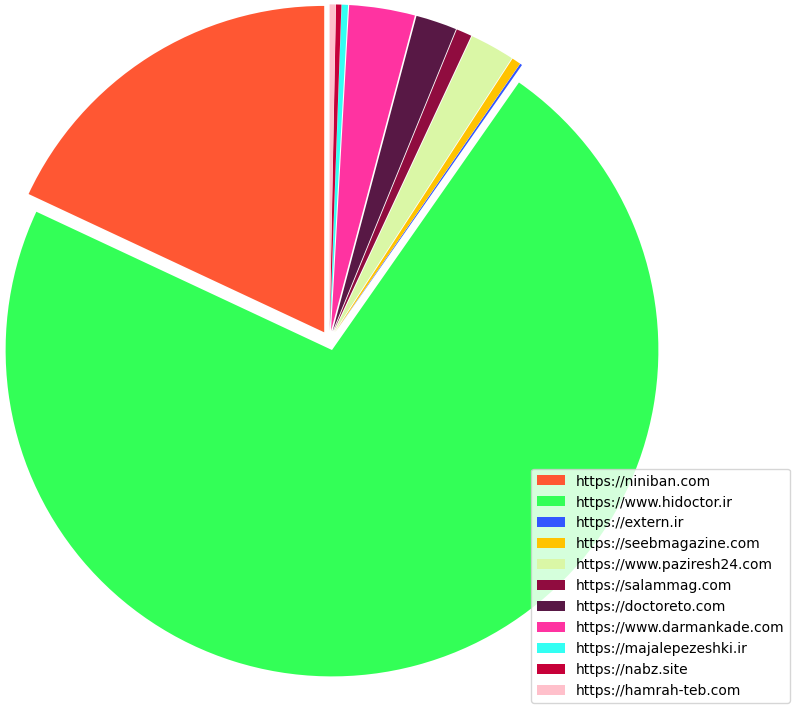
\includegraphics[width=0.4\textwidth]{fig1.png}}
	\caption{Share of articles by magazine}
	\label{fig1}
\end{figure}

\subsection{dataset}
In our research, we crawled more than 140,000 question-answer pairs from Persian medical forums, employing both manual and automatic filtering methods to refine the dataset. This approach is similar to the work done by Yunxiang Li et al
\cite{b6}
. in their article on the Chat Doctor medical language model, where they extracted data from English medical forums. Notably, Yunxiang Li discarded about half of the question-answer pairs based on the length of the answers, as shorter responses are generally inadequate for training a model. However, we faced a greater challenge; Persian doctors tend to provide much shorter answers compared to their English counterparts, resulting in the necessity to discard over 80\% of our question-answer records to ensure quality and relevance for our training purposes.

\section{Training}
\subsection{fine tuning}
We fine-tuned the aya-expanse8b model on 60\% of our corpus, leveraging LoRA
\cite{b12}
method to optimize performance. Specifically, we implemented a rank of 8, an alpha value of 16, and a LoRA dropout rate of 0.05, conducting the fine-tuning for a single epoch. This approach allowed us to effectively adapt the model to our specific dataset while minimizing resource usage, ensuring a balance between efficiency and performance enhancement in our training process.
\subsection{instruction tuning}
In addition to fine-tuning the aya-expanse8b model, we also instruction-tuned the fine-tuned model on our crawled free-form Farsi question-answering (MF3QA) dataset. For this instruction tuning, we employed a LoRA method with a rank of 2, an alpha value of 2, and a LoRA dropout rate of 0.4, conducting the process for a single epoch. This targeted approach allowed us to further enhance the model’s ability to understand and generate responses in the context of Farsi question-answering, optimizing its performance for our specific dataset and improving its overall effectiveness.
\subsection{Carbon Footprint}
During our recent computational experiments, we utilized an A100 PCIe 40/80G hardware setup on the Google Cloud Platform, specifically in the asia-east1 compute region. The hardware was operational for a total of 19 hours, resulting in a carbon footprint of 2.66 kg CO2 equivalent emissions calculated  based on the formula introduced by Wu et all
\cite{b13}
.
\section{Results}
Since there is no publicly available medical Persian language model to compare our results against, and given that only a few small Persian language models exist, we opted to compare our model with a pipeline system that combines an English medical language model with a translator, specifically targeting systems with a total of less than 8 billion parameters, which we define as runnable on home devices. We evaluated our model against two different pipeline configurations to demonstrate that, in addition to their poor grammatical performance, these systems also struggle to effectively encode medical knowledge, as evidenced by their low scores in multiple-choice question-answering datasets. The first configuration involved using MedMobile
\cite{b9}
as the English small medical language model paired with gemma-2b-it
\cite{b14}
as the translator, while the second configuration used MedMobile with Parsinlu
\cite{b15}
\cite{b16}
as the translator. Our comparisons highlighted the limitations of these pipeline systems in both linguistic accuracy and medical comprehension.
\footnote{
	you can see the detailed result at https://github.com/Mehrdadghassabi/Gaokerena
}
\subsection{multiple choice question answering}
In our results section, we address the significant challenge of the lack of available Persian datasets for medical language processing. To overcome this, we translated the medical portion of the Massive Multitask Language Understanding (MMLU)
\cite{b17}
dataset into Persian and supplemented it with data from the Iranian Basic Medical Sciences Entrance Exam(IBMSEE), which we also crawled. Notably,as you can see on Table I our model achieved remarkable success by surpassing the passing score of the Iranian Basic Medical Sciences Entrance Exam, which stands at 36\%, making it the first Persian small language model to pass this exam. Furthermore, our model demonstrated substantial improvements on the translated MMLU dataset, not only achieving higher average scores but also excelling across most sub-categories, thereby showcasing its effectiveness in understanding and generating medical knowledge in the Persian language.
\begin{table}[ht]
	\centering
	\caption{Results on medical multiple choice question answering}
	\begin{tabular}{|l|c|c|c|c|}  % Using vertical lines for a simple table
		\hline
		\textbf{} & \textbf{Gao-} & \textbf{aya-}
		 & \textbf{MedMobile} & \textbf{MedMobile} \\ 
		 & \textbf{kerena} & \textbf{expanse8b} & + \textbf{gemma2b-it} & \textbf{+ parsinlu} \\
		 & (ours) & (baseline) &  &  \\ \hline
		MMLU- & \textbf{48.14} & 40.74 & 14.07 & 25.18 \\ 
		anatomy(fa) &  &  &  &  \\ \hline
		MMLU- & 46.0 & \textbf{49.0} & 20.0 & 35.0 \\
		medical &  &  &  &  \\ 
		genetics(fa) &  &  &  &  \\ \hline
		MMLU- & 43.93 & \textbf{44.51} & 19.08 & 27.17 \\
		college &  &  &  &  \\
		medicine(fa) &  &  &  &  \\ \hline
		MMLU- & \textbf{55.47} & 52.07 & 27.54 & 31.7 \\
		clinical&  &  &  &  \\
		knowledge(fa)&  &  &  &  \\ \hline
		MMLU- & ? & ? & ? & ? \\
        professional&  &  &  &  \\ 
        medicine(fa)&  &  &  &  \\ \hline
        MMLU- & ? & ? & ? & ? \\
        college&  &  &  &  \\
        biology(fa)&  &  &  &  \\ \hline
        MMLU(avg) & ? & ? & ? & ? \\ \hline
		IBMSEE & \textbf{38.69} & 34.52 & 24.40 & 32.73 \\ 
        \hline
	\end{tabular}
	\label{tab:model_results}
\end{table}
\subsection{free form question answering}
\subsubsection{K-QA benchmark}
In this study, we utilized the K-QA dataset introduced by Itay Manes
\cite{b18}
, which consists of expert-generated question-answer pairs, each accompanied by “nice to have” and “must have” lists. Manes proposed two key metrics, Completeness and Factuality, which are essential for evaluating the quality of the question-answer pairs. These metrics, as reformulated by Hyunjae Kim
\cite{b8}
, are defined as follows:  
\[
S_{comp}(r_i,A_i^{\prime}) =  \sum_{a \in A_i^{\prime}} \frac{[r_i \: entails \: a]}{|A_i^{\prime}|}
\]
\[
S_{fact}(r_i,A_i^{\prime}) = 
\begin{cases} 
	0 & \text{if } \exists a \in A_i \: s.t.  \: r_i \: contradicts \: a\\ 
	1 & otherwise
\end{cases}
\]
Manes likened these metrics to traditional precision and recall, leading to the introduction of a new metric, the $F_{1}^{\prime}$ score, analogous to the $F_{1}$ score, defined as: 
\[
F_{1}^{\prime} = \frac{2 \times S_{comp} \times S_{fact}}{S_{comp} + S_{fact}}
\]
In our research, we translated the k-QA dataset into Persian and computed the Completeness and Factuality scores for our model, Gaokerena, as well as for the baseline model,aya-expanse-8b. as you can see in the Table II the results indicated that Gaokerena slightly outperformed aya-expanse-8b in both the $F_{1}^{\prime}$ score and the Factuality score, demonstrating the effectiveness of our approach.

\begin{table}[ht]
	\centering
	\caption{Results on k-qa benchmark}
	\begin{tabular}{|c|c|c|} % l for left-aligned, c for centered
		\hline
		\textbf{} & \textbf{gaokerena} & \textbf{aya-expanse-8b} \\ 
		\hline
		$S_{comp}$ & 0.7194 & \textbf{0.7322} \\ 
		\hline
		$S_{fact}$ & \textbf{0.4925} & 0.4776 \\ 
		\hline
		$F_{1}^{\prime}$ & \textbf{0.5847} & 0.5781 \\ 
		\hline
	\end{tabular}
	\label{tab:model_accuracy}
\end{table}

\subsubsection{AI Evaluating AI}
In addition to our k-QA benchmark, we also utilized GPT-4o
\cite{b19}
as an evaluator for free form question answering. We provided the test set from the MF3QA dataset to both aya-expanse-8b and our model. As illustrated in figure
\ref{fig2}
,GPT-4o predominantly preferred the responses generated by our model to the baseline model. This indicates that our model delivers high-quality responses as judged by an advanced language model.

\begin{figure}[htbp]
	\centerline{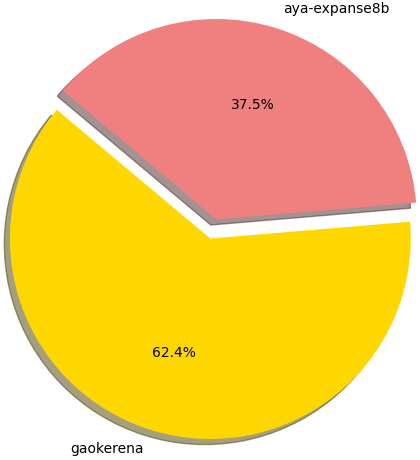
\includegraphics[width=0.4\textwidth]{fig2.png}}
	\caption{GPT-4o choice}
	\label{fig2}
\end{figure}
\section*{Acknowledgment}
We would like to thank Amir Jahani for his help with the data cleaning process.


\begin{thebibliography}{00}
\bibitem{b1} Vaswani, Ashish, et al. "Attention is all you need." Advances in neural information processing systems 30 (2017).
\bibitem{b2} Singhal, Karan, et al. "Toward expert-level medical question answering with large language models." Nature Medicine (2025): 1-8.
\bibitem{b3}
Singhal, Karan, et al. "Large language models encode clinical knowledge." Nature 620.7972 (2023): 172-180.
\bibitem{b4} Taghizadeh, Nasrin, et al. "SINA-BERT: a pre-trained language model for analysis of medical texts in Persian." arXiv preprint arXiv:2104.07613 (2021).
\bibitem{b5} Dang, John, et al. "Aya expanse: Combining research breakthroughs for a new multilingual frontier." arXiv preprint arXiv:2412.04261 (2024).
\bibitem{b6} Li, Yunxiang, et al. "Chatdoctor: A medical chat model fine-tuned on a large language model meta-ai (llama) using medical domain knowledge." Cureus 15.6 (2023).
\bibitem{b7} Touvron, Hugo, et al. "Llama: Open and efficient foundation language models." arXiv preprint arXiv:2302.13971 (2023).
\bibitem{b8} Kim, Hyunjae, et al. "Small language models learn enhanced reasoning skills from medical textbooks." arXiv preprint arXiv:2404.00376 (2024).
\bibitem{b9} Vishwanath, Krithik, et al. "MedMobile: A mobile-sized language model with expert-level clinical capabilities." arXiv preprint arXiv:2410.09019 (2024).
\bibitem{b10} Team, Gemma, et al. "Gemma: Open models based on gemini research and technology." arXiv preprint arXiv:2403.08295 (2024).
\bibitem{b11} Rostami, Pedram, Ali Salemi, and Mohammad Javad Dousti. "Persianmind: A cross-lingual persian-english large language model." arXiv preprint arXiv:2401.06466 (2024).
\bibitem{b12} Hu, Edward J., et al. "Lora: Low-rank adaptation of large language models." ICLR 1.2 (2022): 3.
\bibitem{b13} Wu, Carole-Jean, et al. "Sustainable ai: Environmental implications, challenges and opportunities." Proceedings of Machine Learning and Systems 4 (2022): 795-813.
\bibitem{b14} Team, Gemma, et al. "Gemma 2: Improving open language models at a practical size, 2024." URL https://arxiv. org/abs/2408.00118 1.3 (2024).
\bibitem{b15} Khashabi, Daniel, et al. "Parsinlu: a suite of language understanding challenges for persian." Transactions of the Association for Computational Linguistics 9 (2021): 1147-1162.
\bibitem{b16} Kashefi, Omid. "MIZAN: a large persian-english parallel corpus." arXiv preprint arXiv:1801.02107 (2018).
\bibitem{b17} Hendrycks, Dan, et al. "Measuring massive multitask language understanding." arXiv preprint arXiv:2009.03300 (2020).
\bibitem{b18} Manes, Itay, et al. "K-qa: A real-world medical q\&a benchmark." arXiv preprint arXiv:2401.14493 (2024).
\bibitem{b19} Hurst, Aaron, et al. "Gpt-4o system card." arXiv preprint arXiv:2410.21276 (2024).
\end{thebibliography}


\end{document}
